\documentclass[10pt,a4paper]{article}

\usepackage[utf8]{inputenc}
\usepackage[T1]{fontenc}
\usepackage{lmodern}
\usepackage{microtype}
\usepackage{eurosym}
\usepackage{amssymb}
\usepackage[top=10mm, bottom=12mm, left=12mm, right=12mm, headheight=14pt, footskip=14pt]{geometry}
\usepackage{graphicx}
\usepackage{xcolor}
\usepackage{booktabs}
\usepackage{tabularx}
\usepackage{enumitem}
\usepackage{fancyhdr}
\usepackage[colorlinks=true, linkcolor=blue!70!black, urlcolor=blue!70!black, citecolor=blue!70!black]{hyperref}
\usepackage{tcolorbox}
\tcbuselibrary{skins}

% Colors
\definecolor{europressred}{HTML}{DC2626}
\definecolor{europressdark}{HTML}{0F172A}
\definecolor{techblue}{HTML}{0284C7}
\definecolor{techpurple}{HTML}{7C3AED}
\definecolor{techgreen}{HTML}{059669}
\definecolor{bannergray}{HTML}{F1F5F9}
\definecolor{bordergray}{HTML}{CBD5E1}
\definecolor{cardbg}{HTML}{FFFFFF}

% Configure page headers and footers
\pagestyle{fancy}
\fancyhf{}
\renewcommand{\headrulewidth}{0pt}
\renewcommand{\footrulewidth}{0.4pt}

\newcommand{\headerbar}[3]{%
  \begin{tcolorbox}[colback=europressdark, colframe=europressdark, arc=3pt, leftrule=5pt, colbacktitle=europressdark, coltitle=white, boxsep=1pt, left=6pt, right=6pt, top=4pt, bottom=4pt, borderline west={4pt}{0pt}{#2}]
    \begin{minipage}[c]{0.74\textwidth}
      {\fontsize{10.5pt}{12pt}\selectfont \textbf{\color{white}EUROPRESS SMART-WEIGHT --- #1}}\\[1pt]
      {\fontsize{7pt}{8.5pt}\selectfont \color{gray!40}#3}
    \end{minipage}%
    \hfill
    \begin{minipage}[c]{0.24\textwidth}
      \raggedleft
      \colorbox{#2}{\fontsize{6.5pt}{7.5pt}\selectfont\color{white}\textbf{\MakeUppercase{\thepage\ OF 4}}}%
      \\[1.5pt]
      {\fontsize{6pt}{7pt}\selectfont \color{gray!30}Since AI Hackathon 2026}
    \end{minipage}
  \end{tcolorbox}
  \vspace{-4pt}
}

\newcommand{\conceptbanner}[5]{%
  \begin{tcolorbox}[colback=bannergray, colframe=bordergray, arc=3pt, leftrule=4pt, boxsep=1pt, left=6pt, right=6pt, top=3pt, bottom=3pt, borderline west={3.5pt}{0pt}{#1}]
    \begin{minipage}[c]{0.56\textwidth}
      {\fontsize{8pt}{9.5pt}\selectfont \textbf{\color{europressdark}#2}}
    \end{minipage}%
    \hfill
    \begin{minipage}[c]{0.42\textwidth}
      \raggedleft
      \colorbox{#3}{\fontsize{6pt}{7pt}\selectfont\color{white}\textbf{#4}} \hspace{1pt}
      \colorbox{europressdark}{\fontsize{6pt}{7pt}\selectfont\color{white}\textbf{#5}}
    \end{minipage}
  \end{tcolorbox}
  \vspace{-3pt}
}

% Set itemize spacing
\setlist[itemize]{leftmargin=12pt, labelsep=4pt, topsep=1pt, parsep=0pt, itemsep=1.8pt}
\setlist[enumerate]{leftmargin=14pt, labelsep=4pt, topsep=1pt, parsep=0pt, itemsep=1.5pt}

\begin{document}

% =====================================================================
% PAGE 1: EXECUTIVE SUMMARY (OPTIONS 1 & 2)
% =====================================================================
\rfoot{\fontsize{6.5pt}{7.5pt}\selectfont \textbf{Page 1 / 4 $\cdot$ Executive Summary}}
\lfoot{\fontsize{6pt}{7pt}\selectfont \color{gray!80}Production Options for COMBI and DUO. Full line-item BOM and installation steps in Engineering Appendix (Pages 3--4).}

\headerbar{EXECUTIVE CONCEPT SPECIFICATION}{europressred}{Part I: Plain-Language Overview $\cdot$ Production Options for COMBI ($\le$22\,m$^3$) \& DUO ($\le$30\,m$^3$) Compactors}

\conceptbanner{techblue}{OPTION 1 --- Zero-Hardware Virtual Sensor: Compaction Energy \& Rebound}{techgreen}{\euro{}0 Hardware BOM}{$\pm$8--10\% Accuracy}

\begin{tcolorbox}[colback=white, colframe=bordergray, arc=3pt, boxsep=2pt, left=6pt, right=6pt, top=4pt, bottom=4pt]
\begin{minipage}[t]{0.56\textwidth}
  {\fontsize{7.8pt}{9pt}\selectfont \textbf{\color{techblue}1A. SYSTEM DESCRIPTION \& HOW IT WORKS}}\\[2pt]
  {\fontsize{7.2pt}{9.2pt}\selectfont
  \begin{itemize}
    \item \textbf{Zero Hardware Needed:} 100\% software-only upgrade inside the existing SMART PLC using signals already measured on every compactor (hydraulic cylinder pressure transducer and piston cycle timer).
    \item \textbf{Forward Compaction Work:} Measures the cumulative mechanical energy delivered by the hydraulic ram across all packing strokes. Denser, heavier waste requires higher mechanical work per cubic meter.
    \item \textbf{Decompression Rebound Speed:} When the ram retracts at stroke end, compressed waste pushes back. Springy, dry cardboard rebounds fast (.050\,s); dense, wet waste relaxes slowly.
    \item \textbf{Mass Calculation:} Combines stroke work and rebound relaxation rate with known compactor fill volume (tracked within $\pm$4--5\% by SMART) to determine bulk payload weight.
    \item \textbf{Key Metrics:} \textbf{\euro{}0.00 BOM} $\cdot$ Remote over-the-air (OTA) push via 4G modem (0 technician visits) $\cdot$ \textbf{$\pm$8--10\% accuracy} (ideal for fill alerts, dispatch timing, and sorting contamination triggers).
  \end{itemize}
  }
\end{minipage}%
\hfill
\begin{minipage}[t]{0.42\textwidth}
  \begin{tcolorbox}[colback=europressdark, colframe=bordergray, arc=2pt, boxsep=1pt, left=2pt, right=2pt, top=2pt, bottom=2pt]
    {\fontsize{6.2pt}{7.2pt}\selectfont \color{techblue!40}\textbf{FIG 1.1: HYDRAULIC WORK \& RELAXATION SIGNATURE}\hfill PLC: 50\,Hz}\\[2pt]
    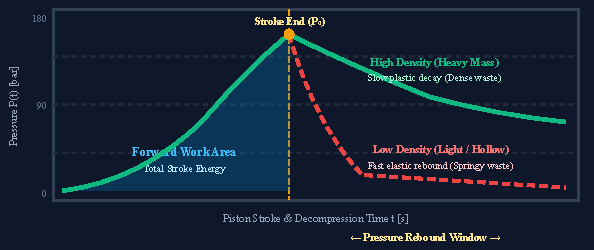
\includegraphics[width=\textwidth]{figures/fig1_hydraulic_signature.pdf}
  \end{tcolorbox}
\end{minipage}
\end{tcolorbox}
\vspace{-3pt}

\conceptbanner{europressred}{OPTION 2 --- Modular Heavy-Duty Shear Pins \& Rail Pads (Direct Mechanical Weighing)}{europressred}{\euro{}192 / \euro{}212 BOM}{$\pm$1.3\% ($1\sigma$) / $\pm$2.6\% (95\%)}

\begin{tcolorbox}[colback=white, colframe=bordergray, arc=3pt, boxsep=2pt, left=6pt, right=6pt, top=4pt, bottom=4pt]
{\fontsize{7.8pt}{9pt}\selectfont \textbf{\color{europressred}2A. SYSTEM DESCRIPTION \& HOW IT WORKS}}\\[2pt]
\begin{minipage}[t]{0.49\textwidth}
  {\fontsize{7.2pt}{9.2pt}\selectfont
  \begin{itemize}
    \item \textbf{Heavy-Duty Industrial Load Cells:} Replaces factory roller axles with 10-tonne stainless steel shear pins (COMBI) or stationary guide-rail wheel pads (DUO). Engineered to withstand 35--40 tonnes of ram force and rough hooklift handling (IP68/IP69K sealed).
    \item \textbf{Zero Wires on Swapped Containers:} On DUO compactors (51.7\% of fleet), 100\% of sensors mount permanently on the stationary press locking hooks and guide rails. Swapped containers remain completely unpowered and wire-free.
  \end{itemize}
  }
\end{minipage}%
\hfill
\begin{minipage}[t]{0.49\textwidth}
  {\fontsize{7.2pt}{9.2pt}\selectfont
  \begin{itemize}
    \item \textbf{Dynamic Tilt \& Weight-Transfer Model:} An onboard 3-axis industrial IMU continuously compensates for loading bay slope (1$^\circ$--4$^\circ$) and center-of-gravity shifts as waste packs rearward. Compaction recoil is gated for 60 seconds post-stroke.
    \item \textbf{Key Metrics:} \textbf{\euro{}192 (COMBI) / \euro{}212 (DUO) OEM BOM} $\cdot$ Installed with a 10t bottle jack during routine annual maintenance $\cdot$ \textbf{$\pm$1.3\% ($1\sigma$) / $\pm$2.6\% at 95\%} ($<$ $\pm$80\,kg on 3 tonnes; flagship for hauler invoice audits).
  \end{itemize}
  }
\end{minipage}
\end{tcolorbox}
\vspace{-3pt}

\begin{tcolorbox}[colback=europressdark, colframe=bordergray, arc=2pt, boxsep=1pt, left=3pt, right=3pt, top=2pt, bottom=2pt]
  {\fontsize{6.2pt}{7.2pt}\selectfont \color{techblue!40}\textbf{FIG 1.2: SENSOR PLACEMENT \& STRUCTURAL INTEGRATION: COMBI MONOBLOCK \& DUO STATIONARY}\hfill RATING: FLINTEC 10t}\\[2pt]
  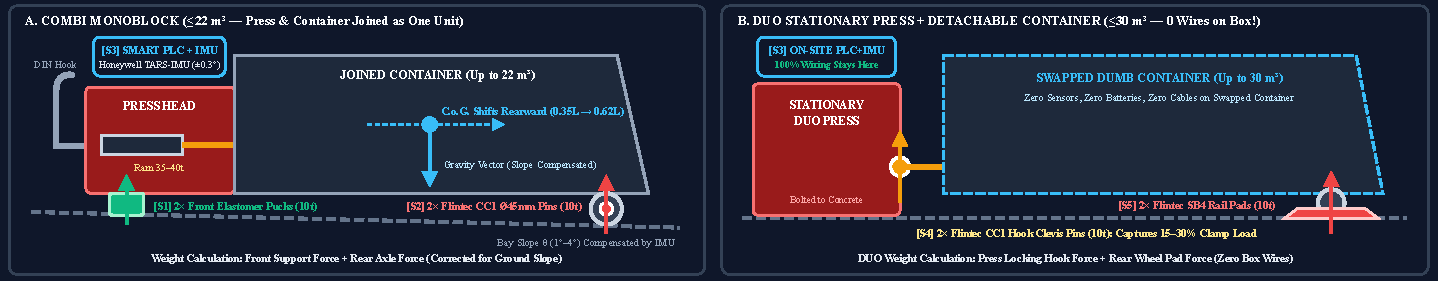
\includegraphics[width=\textwidth]{figures/fig2_cad_subframe_elevation.pdf}
\end{tcolorbox}

\clearpage

% =====================================================================
% PAGE 2: EXECUTIVE SUMMARY (OPTION 3 - THE WILD CARD)
% =====================================================================
\rfoot{\fontsize{6.5pt}{7.5pt}\selectfont \textbf{Page 2 / 4 $\cdot$ Wild Card}}
\lfoot{\fontsize{6pt}{7pt}\selectfont \color{gray!80}Option 3 Non-Contact RF Tomography. Full line-item BOM and installation steps in Engineering Appendix (Pages 3--4).}

\headerbar{EXECUTIVE CONCEPT SPECIFICATION}{techpurple}{Part I: Plain-Language Overview $\cdot$ The Wild Card (Option 3): Non-Contact RF Tomography \& Moisture}

\conceptbanner{techpurple}{OPTION 3 --- Dense On-Metal PIFA RFID Array: Simultaneous Dry Weight \& Moisture}{techpurple}{\euro{}124 Press BOM}{$\pm$5--7\% Mass $\cdot$ $\pm$2.5\% Moisture}

\begin{tcolorbox}[colback=white, colframe=bordergray, arc=3pt, boxsep=2pt, left=6pt, right=6pt, top=4pt, bottom=4pt]
{\fontsize{7.8pt}{9pt}\selectfont \textbf{\color{techpurple}3A. CORE IDEA: WHY RFID BEATS ACOUSTIC SENSORS WHEN VOLUME IS ALREADY KNOWN ($\pm$5\%)}}\\[2pt]
\begin{minipage}[t]{0.49\textwidth}
  {\fontsize{7.2pt}{9.2pt}\selectfont
  \begin{itemize}
    \item \textbf{Building on Known Volume:} Acoustic sensors only measure air headspace (occupied volume)---which Europress SMART \textbf{already knows within $\pm$4--5\%}. Weight equals Volume $\times$ Density. We only need to measure material density!
    \item \textbf{Safe Radio Wave Penetration (868\,MHz):} Safe high-frequency radio waves travel cleanly through dry non-metallic recyclables (cardboard, paper, plastics) inside the steel container.
    \item \textbf{The Recycler's Dilemma (Scenario S28):} Conventional scales record total gross weight. A 3,000\,kg cardboard load holding \textbf{2,200\,kg dry fiber + 800\,kg rainwater} is weighed as 3,000\,kg, causing paper-mill quality downgrades or load rejections.
  \end{itemize}
  }
\end{minipage}%
\hfill
\begin{minipage}[t]{0.49\textwidth}
  {\fontsize{7.2pt}{9.2pt}\selectfont
  \begin{itemize}
    \item \textbf{Two Measurements from One Signal:}
      \begin{itemize}[label=--, leftmargin=8pt, itemsep=1pt]
        \item \textbf{Wave Speed Delay:} Packed dry material slows radio waves $\rightarrow$ measures \textbf{Dry Recyclable Mass}.
        \item \textbf{Signal Energy Absorption:} Water absorbs radio energy strongly $\rightarrow$ measures \textbf{Moisture Content \& Water Weight}.
      \end{itemize}
    \item \textbf{Solving the Steel Box:} 16 On-Metal PIFA tags recessed in plastic wear rails along inner walls; steel wall acts as a signal booster (+3\,dBi). Tag \#1 auto-reads \textbf{Container ID \& Tare}.
    \item \textbf{Key Metrics:} \textbf{\euro{}124 per press} (\euro{}40 / container) $\cdot$ Bolt-on rail + plug reader into PLC $\cdot$ \textbf{$\pm$5--7\% weight, $\pm$2.5\% moisture}.
  \end{itemize}
  }
\end{minipage}
\end{tcolorbox}
\vspace{-3pt}

\begin{tcolorbox}[colback=europressdark, colframe=bordergray, arc=2pt, boxsep=1pt, left=3pt, right=3pt, top=2pt, bottom=2pt]
  {\fontsize{6.2pt}{7.2pt}\selectfont \color{techpurple!40}\textbf{FIG 2.1: APERTURE-COUPLED ON-METAL PIFA RFID TOMOGRAPHY \& WEAR RAIL INTEGRATION}\hfill ETSI: 865--868\,MHz}\\[2pt]
  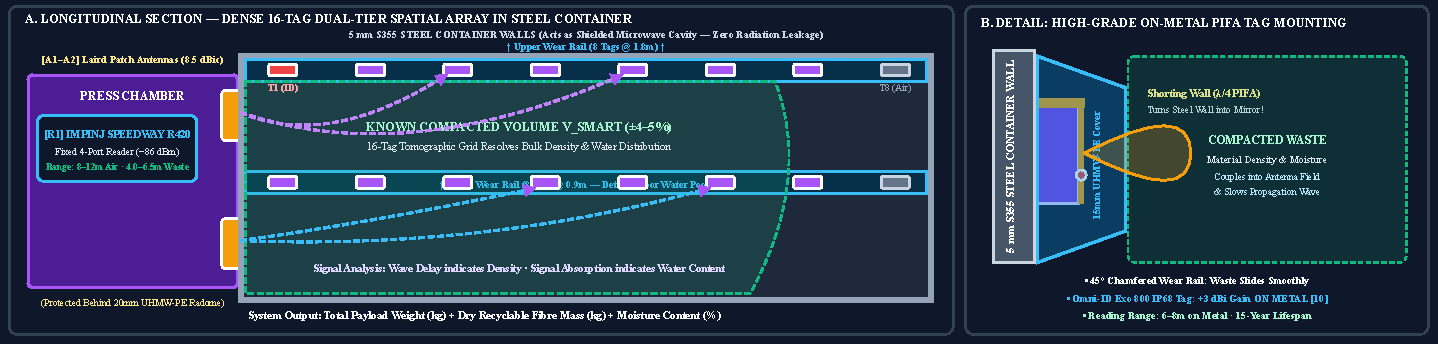
\includegraphics[width=\textwidth]{figures/fig3_rfid_aperture_tomography.pdf}
\end{tcolorbox}
\vspace{-3pt}

\begin{tcolorbox}[colback=techpurple!5, colframe=techpurple!40, arc=3pt, boxsep=2pt, left=6pt, right=6pt, top=4pt, bottom=4pt]
{\fontsize{7.8pt}{9pt}\selectfont \textbf{\color{techpurple}3B. RESEARCH-TO-BUSINESS (R2B) VALUE BEYOND WASTE}}\\[2pt]
\begin{minipage}[t]{0.49\textwidth}
  {\fontsize{7.2pt}{9.2pt}\selectfont
  \begin{itemize}
    \item \textbf{Paper-Mill Quality Shield (Waste):} Flags rain/snow moisture inside cardboard before pickup, protecting Grade-A circular economy rebates and preventing customer clawback disputes.
    \item \textbf{Automated DUO Container Tare Tracking:} Reads container serial tag on docking and retrieves exact certified steel tare weight (2,100--2,600\,kg) from the cloud database.
  \end{itemize}
  }
\end{minipage}%
\hfill
\begin{minipage}[t]{0.49\textwidth}
  {\fontsize{7.2pt}{9.2pt}\selectfont
  \begin{itemize}
    \item \textbf{Nordic Forestry \& Bioenergy (UPM, Metsä, Stora Enso):} Measures \textbf{bone-dry woodchip tonnage (MWh heating value)} vs. water weight on timber trucks without 24h oven drying!
    \item \textbf{Europress Balex Balers:} Embedding a \euro{}0.15 passive tag into each finished bale gives recycling mills instant dry weight \& moisture data directly on the forklift.
  \end{itemize}
  }
\end{minipage}
\end{tcolorbox}

\clearpage

% =====================================================================
% PAGE 3: ENGINEERING APPENDIX (PART 1 - BOM & INSTALLATION)
% =====================================================================
\rfoot{\fontsize{6.5pt}{7.5pt}\selectfont \textbf{Page 3 / 4 $\cdot$ Appendix Part 1}}
\lfoot{\fontsize{6pt}{7pt}\selectfont \color{gray!80}Component datasheets based on Flintec Inc., Impinj Speedway R420, and Omni-ID Exo 800.}

\headerbar{ENGINEERING APPENDIX (PART 1)}{techgreen}{Itemized Bill of Materials (BOM), COTS Component Datasheet Specifications \& Retrofit Protocols}

\conceptbanner{techgreen}{APPENDIX SECTION 1 --- Itemized Bill of Materials (BOM) \& Manufacturer Datasheets}{techgreen}{1,000+ OEM Volume}{IP68/IP69K Sealed}

\begin{tcolorbox}[colback=white, colframe=bordergray, arc=3pt, boxsep=2pt, left=5pt, right=5pt, top=3pt, bottom=3pt]
{\fontsize{7.5pt}{8.5pt}\selectfont \textbf{\color{europressred}A1. Option 2 Modular Mechanical Kit: Component Specifications \& Datasheet Ratings}}\\[2pt]
{\fontsize{6.5pt}{7.8pt}\selectfont
\begin{tabularx}{\textwidth}{l p{2.2cm} p{1.8cm} X c r}
\toprule
\textbf{Subsystem} & \textbf{Component Model} & \textbf{Manufacturer} & \textbf{Datasheet Ratings \& Environmental Spec} & \textbf{Qty} & \textbf{OEM Cost} \\
\midrule
\textbf{Rear Load Pins (COMBI)} & Type CC1 / WTS 10t & Flintec / Interface & Ø45\,mm 17-4PH stainless steel; Rated capacity: \textbf{10 tonnes (100\,kN)}; 150\% safe overload; 300\% break load; IP68/IP69K hermetic laser weld; Operating: \textbf{-40$^\circ$C to +80$^\circ$C}; Error $<$ $\pm$0.25\%. & 2 & \euro{}84.00 \\
\textbf{Rear Rail Pads (DUO)} & Type SB4 / RC3 & Flintec Inc. & Stainless steel shear-beam cell; Rated capacity: \textbf{10 tonnes}; OIML R60 C3 legal-for-trade (3,000\,div); 150\% safe overload; IP68/IP69K laser-welded seal; Temp: -40$^\circ$C to +80$^\circ$C. & 2 & \euro{}104.00 \\
\textbf{Front Pucks (COMBI)} & Custom Load Puck & Europress OEM & Shore-80A elastomer-isolated compression puck; 10t rated vertical load limit; vibration dampening. & 2 & \euro{}76.00 \\
\textbf{Hook Clevis Pins (DUO)} & Type CC1 10t Pin & Flintec Inc. & Instrumented clevis pin inside stationary press locking hook (10t rated, IP69K); captures 15--30\% bridged clamp tension. & 2 & \euro{}76.00 \\
\textbf{Edge Interface PCB} & SMART-Weight Edge & Custom Europress & TI ADS1234 24-bit $\Delta\Sigma$ 4-ch ADC + Honeywell TARS-IMU motion sensor ($\pm$0.3$^\circ$ dynamic tilt); isolated RS-485 Modbus RTU. & 1 & \euro{}18.00 \\
\textbf{Armored Cabling} & Industrial PUR M12 & Lumberg / Phoenix & Heavy-duty braided PUR IP67/IP69K industrial cable harness with chassis P-clips. & 1 & \euro{}14.00 \\
\midrule
\multicolumn{4}{l}{\textbf{TOTAL INDICATIVE OEM BOM (OPTION 2 HARDWARE KIT)}} & \textbf{Kit} & \textbf{\euro{}192 / \euro{}212} \\
\bottomrule
\end{tabularx}
}
\end{tcolorbox}
\vspace{-3pt}

\begin{tcolorbox}[colback=white, colframe=bordergray, arc=3pt, boxsep=2pt, left=5pt, right=5pt, top=3pt, bottom=3pt]
{\fontsize{7.5pt}{8.5pt}\selectfont \textbf{\color{techpurple}A2. Option 3 Dense On-Metal PIFA RFID Array: Component Specifications \& Datasheet Ratings}}\\[2pt]
{\fontsize{6.5pt}{7.8pt}\selectfont
\begin{tabularx}{\textwidth}{l p{2.2cm} p{1.8cm} X c r}
\toprule
\textbf{Subsystem} & \textbf{Component Model} & \textbf{Manufacturer} & \textbf{Datasheet Ratings \& Environmental Spec} & \textbf{Qty} & \textbf{OEM Cost} \\
\midrule
\textbf{UHF RFID Reader} & Speedway R420 & Impinj / Zebra & Fixed 4-port industrial UHF interrogator; ETSI 865--868\,MHz; sensitivity -86\,dBm; power +31.5\,dBm (1.4\,W conducted); die-cast aluminum IP65/IP67 enclosure (-20$^\circ$C to +55$^\circ$C); Modbus/RS-485. & 1 & \euro{}62.00 \\
\textbf{Aperture Antennas} & S9028PCL / A5020 & Laird / Times-7 & Circularly-polarized planar patch antenna; 8.5\,dBic gain; 68$^\circ$ beamwidth; heavy-duty IP67 housing behind 20\,mm UHMW-PE radome in press throat. & 2 & \euro{}22.00 \\
\textbf{On-Metal PIFA Tags} & Exo 800 / Steelwave & Omni-ID / Confidex & High-impact thermoplastic IP68/IP69K on-metal tags; +3\,dBi directional gain on steel; 8--12\,m free-air range; 4.0--6.5\,m penetration through packed waste; passive (15+ yr lifespan). & 16 & \euro{}24.00 \\
\textbf{Protective Wear Rails} & Machined UHMW-PE & Europress OEM & 15\,mm thick chamfered wear rail (left and right walls); low friction (0.10) ensures trash slides over smoothly without contacting tags. & 2 & \euro{}16.00 \\
\midrule
\multicolumn{4}{l}{\textbf{TOTAL INDICATIVE OEM BOM (OPTION 3 RF ARRAY)}} & \textbf{Kit} & \textbf{\euro{}124.00} \\
\bottomrule
\end{tabularx}
}
\end{tcolorbox}
\vspace{-3pt}

\conceptbanner{techblue}{APPENDIX SECTION 2 --- Mechanical \& Electrical Installation Protocols}{techblue}{Zero Civil Work}{Bottle Jack Only}

\begin{tcolorbox}[colback=white, colframe=bordergray, arc=3pt, boxsep=2pt, left=5pt, right=5pt, top=3pt, bottom=3pt]
\begin{minipage}[t]{0.48\textwidth}
  {\fontsize{7.2pt}{8.2pt}\selectfont \textbf{\color{techblue}A3-1. Option 1 Software Deployment}}
  {\fontsize{6.8pt}{8.2pt}\selectfont
  \begin{itemize}
    \item \textbf{Remote OTA Deployment:} Connect to compactor SMART PLC via existing onboard 4G/LTE gateway.
    \item \textbf{Firmware Provisioning:} Flash updated PLC program containing Forward Compaction Work routines and Peleg--Moreyra relaxation time-decay algorithms.
    \item \textbf{Telemetry Tag Activation:} Provision cloud variables (\texttt{mass\_predicted\_kg}, \texttt{density\_bulk\_kg\_m3}, \texttt{rebound\_tau\_s}). 0 technician visits.
  \end{itemize}
  }
  \vspace{2pt}
  {\fontsize{7.2pt}{8.2pt}\selectfont \textbf{\color{techpurple}A3-3. Option 3 (RFID) Installation}}
  {\fontsize{6.8pt}{8.2pt}\selectfont
  \begin{itemize}
    \item \textbf{Wear Rail Fastening:} Fasten pre-drilled UHMW-PE wear rails (with recessed tags) along container interior ribs using M6 countersunk screws.
    \item \textbf{Throat Antenna Mounting:} Fasten 2$\times$ patch antennas behind 20\,mm UHMW-PE radome inside press throat; wire RS-485 Modbus to SMART PLC.
  \end{itemize}
  }
\end{minipage}%
\hfill
\begin{minipage}[t]{0.48\textwidth}
  {\fontsize{7.2pt}{8.2pt}\selectfont \textbf{\color{europressred}A3-2. Option 2 Mechanical Installation Procedure}}
  {\fontsize{6.8pt}{8.2pt}\selectfont
  \begin{itemize}
    \item \textbf{COMBI Monoblock Procedure:}
      \begin{enumerate}
        \item Position mobile 10t hydraulic bottle jack under rear jacking pad.
        \item Elevate rear frame 30\,mm; slide out uninstrumented axle pins.
        \item Insert pre-calibrated Flintec CC1 Ø45\,mm 10t pins; secure snap rings.
        \item Lower frame; place elastomer pucks under front leveling pads.
        \item Route armored M12 harness into junction box; connect Modbus.
      \end{enumerate}
    \item \textbf{DUO Stationary Compactor Procedure:}
      \begin{enumerate}
        \item Anchor 2$\times$ Flintec SB4 10t rail pads onto concrete guide rails along container rear wheel path.
        \item Replace uninstrumented clevis pins on stationary press locking hooks with Flintec CC1 10t instrumented pins.
        \item Route M12 cables into press cabinet. \textbf{Swapped containers require zero sensors, zero wiring, zero batteries, and zero modifications.}
      \end{enumerate}
  \end{itemize}
  }
\end{minipage}
\end{tcolorbox}

\clearpage

% =====================================================================
% PAGE 4: ENGINEERING APPENDIX (PART 2 - BLUEPRINT & METROLOGY)
% =====================================================================
\rfoot{\fontsize{6.5pt}{7.5pt}\selectfont \textbf{Page 4 / 4 $\cdot$ Appendix Part 2}}
\lfoot{\fontsize{6pt}{7pt}\selectfont \color{gray!80}Metrological error model based on RSS formula $\sqrt{\sum \sigma_i^2}$. Factory validation runnable at Europress Kerava facility.}

\headerbar{ENGINEERING APPENDIX (PART 2)}{techgreen}{Master Subframe Blueprint, Executive Decision Matrix, Error Budget \& References}

\begin{tcolorbox}[colback=europressdark, colframe=bordergray, arc=2pt, boxsep=1pt, left=3pt, right=3pt, top=2pt, bottom=2pt]
  {\fontsize{6.2pt}{7.2pt}\selectfont \color{techgreen!40}\textbf{FIG 3.1: MASTER SUBFRAME BLUEPRINT \& MODULAR EDGE-TO-CLOUD ARCHITECTURE}\hfill DIN 30722 RAILS $\cdot$ RS-485 MODBUS RTU}\\[2pt]
  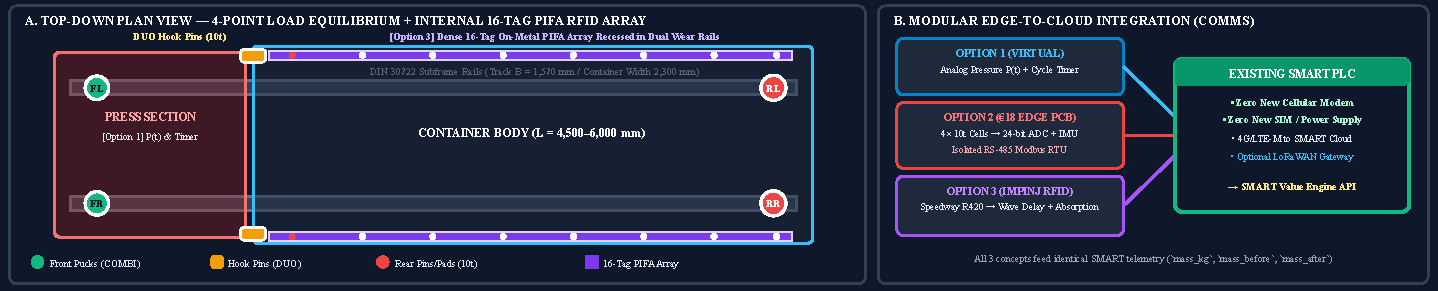
\includegraphics[width=\textwidth]{figures/fig4_master_subframe_plan.pdf}
\end{tcolorbox}
\vspace{-3pt}

\begin{minipage}[t]{0.485\textwidth}
  \begin{tcolorbox}[colback=white, colframe=bordergray, arc=3pt, boxsep=2pt, left=4pt, right=4pt, top=3pt, bottom=3pt]
  {\fontsize{7.2pt}{8.2pt}\selectfont \textbf{\color{europressred}A4. Executive Decision Matrix Across All 3 Options}}\\[2pt]
  {\fontsize{6.4pt}{7.6pt}\selectfont
  \begin{tabularx}{\textwidth}{l p{1.6cm} p{1.7cm} X}
  \toprule
  \textbf{Criteria} & \textbf{Option 1 (Virtual)} & \textbf{Option 2 (Mech)} & \textbf{Option 3 (RFID)} \\
  \midrule
  \textbf{OEM Cost} & \textbf{\euro{}0.00} & \textbf{\euro{}192 / \euro{}212} & \textbf{\euro{}124} (+ \euro{}40/box) \\
  \textbf{Installation} & Remote OTA push & Bottle-jack pin swap & Bolt rail + radome \\
  \textbf{Accuracy} & $\pm$8--10\% & \textbf{$\pm$2.6\%} ($\pm$1.3\% 1$\sigma$) & $\pm$5--7\% wt, $\pm$2.5\% mst \\
  \textbf{DUO Units} & Supported & Supported (0 box wire) & Supported (tare ID) \\
  \textbf{Key Value} & Fill alert triggers & \textbf{Invoice auditing} & Quality shield (S28) \\
  \bottomrule
  \end{tabularx}
  }
  \end{tcolorbox}
\end{minipage}%
\hfill
\begin{minipage}[t]{0.485\textwidth}
  \begin{tcolorbox}[colback=white, colframe=bordergray, arc=3pt, boxsep=2pt, left=4pt, right=4pt, top=3pt, bottom=3pt]
  {\fontsize{7.2pt}{8.2pt}\selectfont \textbf{\color{techblue}A5. Quantitative Error Budget (Option 2 on 3,000\,kg)}}\\[2pt]
  {\fontsize{6.4pt}{7.6pt}\selectfont
  \begin{tabularx}{\textwidth}{l c X r}
  \toprule
  \textbf{Contributor} & \textbf{Raw} & \textbf{Mitigation} & \textbf{Residual ($1\sigma$)} \\
  \midrule
  \textbf{Cell Non-Linearity} & $\pm$0.50\% & 24-bit ADC + 3-pt cal & $\pm$0.45\% (13.5\,kg) \\
  \textbf{C.o.G. Rearward Shift} & $\pm$12.0\% & 4-pt force summation & $\pm$0.55\% (16.5\,kg) \\
  \textbf{DUO Clamp Bridging} & $\pm$18.0\% & Hook pins + 60\,s gate & $\pm$0.75\% (22.5\,kg) \\
  \textbf{Bay Slope (1$^\circ$--4$^\circ$)} & $\pm$0.80\% & TARS-IMU tilt correction & $\pm$0.10\% (3.0\,kg) \\
  \textbf{Thermal Span} & $\pm$1.60\% & Full bridge + auto-tare & $\pm$0.40\% (12.0\,kg) \\
  \midrule
  \multicolumn{3}{l}{\textbf{COMBINED RSS TOTAL ($<$ $\pm$80\,kg on 3\,t)}} & \textbf{$\pm$1.30\% / $\pm$2.60\%} \\
  \bottomrule
  \end{tabularx}
  }
  \end{tcolorbox}
\end{minipage}
\vspace{-3pt}

\begin{minipage}[t]{0.485\textwidth}
  \begin{tcolorbox}[colback=white, colframe=bordergray, arc=3pt, boxsep=2pt, left=4pt, right=4pt, top=3pt, bottom=3pt]
  {\fontsize{7.2pt}{8.2pt}\selectfont \textbf{\color{techgreen}A6. 1-Day Factory Validation Plan ($<$\euro{}1,500)}}\\[2pt]
  {\fontsize{6.3pt}{7.4pt}\selectfont
  \begin{itemize}
    \item \textbf{Hours 0--2 (Setup):} Instrument 1$\times$ CombiMax 20\,m$^3$ and 1$\times$ DuoMax 24\,m$^3$ over reference truck scale ($\pm$5\,kg truth).
    \item \textbf{Hours 2--4 (Deadweight):} Apply 6$\times$ 500\,kg certified test blocks (0 to 3,000\,kg) across Front, Mid, and Rear; verify error $\le$ $\pm$78\,kg.
    \item \textbf{Hours 4--6 (Clamp \& Compaction):} Sweep DUO hook tension (5--25\,t); run 20 full 35\,t strokes on cardboard vs. wet biowaste.
    \item \textbf{Hours 6--8 (Tilt \& Moisture):} Jack chassis side by 3$^\circ$ (verify IMU tilt); spray 100--400\,L water (verify RFID moisture decoupling).
  \end{itemize}
  }
  \end{tcolorbox}
\end{minipage}%
\hfill
\begin{minipage}[t]{0.485\textwidth}
  \begin{tcolorbox}[colback=white, colframe=bordergray, arc=3pt, boxsep=2pt, left=4pt, right=4pt, top=3pt, bottom=3pt]
  {\fontsize{7.2pt}{8.2pt}\selectfont \textbf{\color{europressred}A7. Academic \& Industrial References [1--10]}}\\[2pt]
  {\fontsize{5.6pt}{6.6pt}\selectfont
  \begin{itemize}
    \item \textbf{[1]} Triet, F. et al. (2004), \textit{Control Eng. Practice}, 12(7), 843--853.
    \item \textbf{[2]} Mani, S. et al. (2006), \textit{Biosyst. Eng.}, 95(2), 197--206.
    \item \textbf{[3]} Peleg, M. \& Moreyra, R. (1979), \textit{Powder Tech.}, 23(2), 277--279.
    \item \textbf{[4]} OIML R 60 / EN 45501 (2017), \textit{Metrological Regulation for Load Cells}.
    \item \textbf{[5]} Flintec Inc. (2023), \textit{Type CC1 Load Pin \& Type SB4 Beam Datasheets}.
    \item \textbf{[6]} Cebon, D. (1999), \textit{Handbook of Vehicle-Road Interaction}, CRC Press.
    \item \textbf{[7]} Trabelsi, S. \& Nelson, S. O. (2003), \textit{IEEE Trans. Instrum. Meas.}, 52(6).
    \item \textbf{[8]} Wang, J. et al. (2017), \textit{ACM MobiCom '17}, 288--300.
    \item \textbf{[9]} Buffi, A. et al. (2020), \textit{IEEE Sensors J.}, 20(12), 2315--2324.
    \item \textbf{[10]} Marrocco, G. (2008), \textit{IEEE Antennas \& Propag. Mag.}, 50(1), 66--79.
  \end{itemize}
  }
  \end{tcolorbox}
\end{minipage}

\end{document}
